\documentclass[10pt,dvipdfmx]{jsarticle}
\usepackage{ascmac}
\usepackage[margin=15truemm]{geometry}
\usepackage{amsmath}
\usepackage[dvipdfmx]{graphicx}
\usepackage{subcaption}
\setlength{\columnseprule}{0.3mm}


\begin{document}

\title{信号処理特論 第13回課題}
\author{視覚認知システム研究室\\学籍番号:2433730032 岡村 翼}
\date{\today}
\maketitle

{\textgt{課題3} }
与えられた真値(True)と入力信号x(n)と出力信号y(n)を用いて、最小2乗法により求めた推定値(Estimated)及び誤差(Error)を表1に示す。
    \begin{table}[h]
      \caption{Least squares method}
      \label{a}
      \centering
      \begin{tabular}{|c|c|c|c|} \hline
        & 真値 & 推定値 & 誤差\\ \hline
        $g(0)$ & 1.0 &  1.00220591 &-0.00220591  \\ \hline
        $g(1)$ & -0.9 &  -0.90193319  &0.00193319\\ \hline
        $g(2)$ & 0.8 &  0.8016873 &-0.0016873\\ \hline
        $g(3)$ & -0.7 &  -0.69861888  &-0.00138112 \\ \hline
        $g(4)$ & 0.6 & 0.59849517 &0.00150483\\ \hline
        \end{tabular}
    \end{table}
また、プロットしたものを図\ref{fig:LS1}に示す。\\

  \begin{figure}[h]
    \centering
      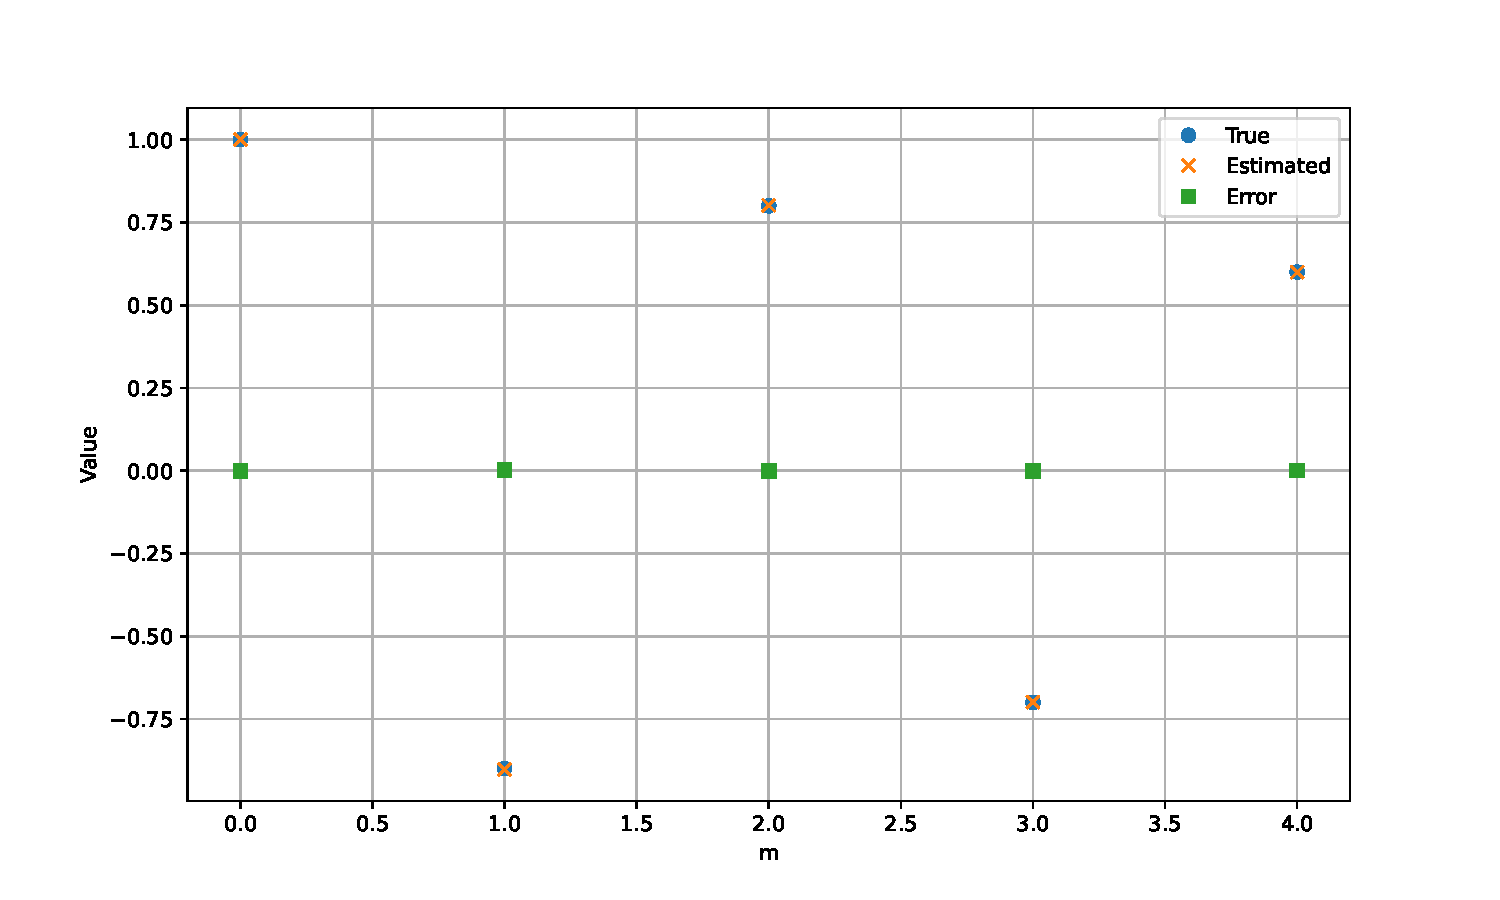
\includegraphics[width=0.8\textwidth]{LS1.pdf}
	\caption{Least squares method}
      \label{fig:LS1}
 \end{figure}
\end{document}